\chapter{The deterministic Lorenz 80 model} \label{cap:ch01_lorenz_deterministic}
\section{Introduction} \label{sec:ch01_introduction}
This chapter aims to present the deterministic Lorenz 80 model. To do so, we begin in section \ref{sec:ch01_geophysics} with an introduction to the basic concepts of geophysics, in order to familiarize the reader with the fundamentals of this area. Next, in section \ref{sec:ch01_model_presentation}, we contextualize the model, discussing the works that preceded it and the motivations behind its formulation.
In section \ref{sec:ch01_shallow_water}, we introduce the shallow water model, which serves as the basis for the development of Lorenz 80. Its construction is detailed in section \ref{sec:ch01_model_construction}, followed by a presentation of its main properties and characteristics in section \ref{sec:ch01_model_properties}. Finally, section \ref{sec:ch01_deterministic_simulations} presents computational simulations performed with the model, accompanied by a graphical analysis of the results.
\section{Brief considerations on geophysics} \label{sec:ch01_geophysics}
In this section, we have compiled a brief glossary of the main concepts of geophysics that serve as a basis for understanding the Lorenz 80 model. Below are the definitions of some fundamental geophysical concepts for the model studied:
\begin{itemize}
    \item \textbf{Quasi-geostrophic.}
    
\item \textbf{Coriolis parameter.}
    \item \textbf{Hydrostatic equilibrium.}
\item \textbf{Stratification.}
\item \textbf{Momentum.}
\item \textbf{Mass conservation.}
\end{itemize}
\section{Motivation and presentation of the model} \label{sec:ch01_model_presentation}
Edward Norton Lorenz (1917-2008) was an important mathematician and meteorologist responsible for publishing several articles and developing models in the field of weather forecasting and other geophysical phenomena.
Among them, the most famous was the Lorenz 63 model, popularly known as the “butterfly effect,” which was a milestone of great relevance for computational mathematical simulations.
In 1980, Lorenz published an article entitled “Attractor Sets and Quasi-Geostrophic Equilibrium” \citep{Lorenz1980}. In it, Lorenz presents the construction and simulation of two distinct models: the first is formed from the{Attractor Sets and Quasi-Geostrophic Equilibrium }" \citep{Lorenz1980}. In it, Lorenz presents the construction and simulation of two distinct models: the first is formed from primitive equations (PE) with nine ODEs (ordinary differential equations), derived from shallow water equations with topography and forcing, while the second is a quasi-geostrophic (QG) model with 3 ODEs, obtained by discarding the variables associated with the divergent flow $x$ and its corresponding terms. The PE model contains both fast gravitational waves and slow quasi-geostrophic oscillations, while the QG model retains only the latter, in a simplified framework for the mid-latitude atmosphere.

\section{The shallow water model} \label{sec:ch01_shallow_water}
The shallow water model describes a fluid of constant density, in hydrostatic equilibrium, which may or may not be rotating. In it, the horizontal scale is significantly larger than the depth. This fluid has a free surface and is bounded by edges. In the case considered, we adopt the single-layer version, which is advantageous because it allows us to disregard the effects of stratification. \citep{Vallis2017}.
Mathematically, to construct the shallow water model, we consider the hydrostatic equilibrium equation, given by:
\begin{equation}
    
\frac{\partial p}{\partial z} = - \rho_0g, \label{eq:equilibrio_hidrostatico}
\end{equation}
where:
\begin{itemize}
    \item $p$: fluid pressure,
    \item $z$: vertical coordinate (positive upwards),
    \item $\rho_0$: constant fluid density,
    \item $g$: acceleration due to gravity.
\end{itemize}
From the manipulations involving the concepts of momentum and mass conservation, detailed in \citet{Vallis2017}, we obtain the equations that describe the model:
\begin{align}
\frac
{\partial V}{\partial t} + (V \cdot \nabla)V + f \mathbf{k} \times V & = -g \nabla z \label{eq:shallow-water-1} \\
    \frac{\partial z}{\partial t} + \nabla \cdot (z V)                        & = 0 \label{eq:shallow-water-2}
    
\end{align}
Where:
\begin{itemize}
    \item $t$: time;
    \item $\mathbf{r}$: initial position vector;
    \item $V(t,r)$: horizontal velocity;
    \item $z(t,r)$: surface height;
    \item $f$: Coriolis parameter;
    
\item $g$: acceleration due to gravity;
    \item $\mathbf{k}$: vertical vector.
\end{itemize}
\section{Model construction} \label{sec:ch01_model_construction}
In this section, we will present the construction of the models presented in the article \citet{Lorenz1980}. As mentioned earlier, the model is constructed from shallow water equations with some particularities described below.
 
Let us consider a homogeneous and incompressible fluid, that is, with constant density throughout the volume and invariable volume even under pressure variations. The flow is predominantly horizontal, described by a velocity $V(t, \mathbf{r})$ independent of height, where $\mathbf{r}$ represents the initial position vector.
The vertical component of velocity is determined by mass continuity. The free surface of the fluid is located at height $H + z(t, \mathbf{r})$, where $H$ represents the average depth and the base rests on a variable topography $h(\mathbf{r})$. We also have that $h(\mathbf{r})$ and $z(t, \mathbf{r})$ have zero mean.
The system is subject to planetary rotation, with a constant Coriolis parameter $f$.
Both the velocity field $V$ and the surface elevation $z$ undergo diffusive dissipation,
associated with small-scale movements: the term $\nu$ represents the viscous diffusion coefficient (momentum dissipation) and $\kappa$ represents the thermal diffusion coefficient. The model also includes an external forcing term $F(\mathbf{r})$ and, finally, the hydrostatic equilibrium hypothesis is adopted.

From the above description, we can construct the following diagram:
\begin{figure}[H]
    \centering
    
\begin{tikzpicture}[scale=1] 
        % Free surface
        \draw[above] (0,4) to[out=0,in=180] (1,4.2)
to[out=0,in=180] (2,3.8)
        to[out=0,in=180] (3.4.2)
        to[out=0,in=180] (4.3.8)
        to[out=0,in=180] (5.4.2)
        to[out=0,in=180] (6.3.8);
        \node[right] at (6.3.8) {Free surface};
                
        % Dashed reference line for z
        \draw[dashed] (2,4.2) -- (1,4.2);
                
        % Deviation of surface z
        \draw[thick] (2,3.8) -- (2,4.2);
        
\draw[thick] (1.9,3.8) -- (2.1,3.8); % lower trace
        \draw[thick] (1.9,4.2) -- (2.1,4.2); % upper trace
        \node[above] at (2,4.3) {$z(t,\mathbf{r})$};
                        
% Velocity V(t,r)
        \node at (2,3) {$ V(t,\mathbf{r}) \rightarrow$};
                
        % Average depth H
        \draw[thick] (4,3.8) -- (4,1.8);
        
\draw[thick] (3.9,3.8) -- (4.1,3.8); % upper trace
        \draw[thick] (3.9,1.8) -- (4.1,1.8); % lower trace
        \node at (4.5,2.8) {$H$};
                        
% Bottom topography (lower curve)
        \draw[dotted, thick] (0,2) to[out=10,in=170] (2,2.3)
 
        to[out=350,in=170] (4,1.8)
        to[out=350,in=170] (6,2);
        
\node[right] at (6,1.9) {Topography of the bottom};
                
        % Variation of topography h
        \draw[thick] (2,2.3) -- (2,1.8);
        \draw[thick] (1.9,2.3) -- (2.1,2.3); % upper trace
        
\draw[thick] (1.9,1.8) -- (2.1,1.8); % lower trace
        \node[below] at (2,1.6) {$h(\mathbf{r})$};
                        
% dashed reference line for h
        \draw[dashed] (2,1.8) -- (4,1.8);
                
    \end{tikzpicture}
    \caption{Diagram of the adapted shallow water model}
    \label{fig:fluid-topography}
\end{figure}
Furthermore, the adapted shallow water model is expressed by:
\begin{align}
    \frac{\partial V}{\partial t} & = - ( V \cdot \nabla)V - f \mathbf{k} \times V - g \nabla z + \nu \nabla^2 V \label{eq:modified-shallow-water-1}     \\
    
\frac{\partial z}{\partial t} & = - (V \cdot \nabla)(z - h) - (H + z - h)\nabla \cdot  V + \kappa \nabla^2 z + F \label{eq:modified-shallow-water-2} 
\end{align}
% Where:
% \begin{multicols}{2}
%     \begin{itemize}
%       \item $t$: time
%       \item $\mathbf{r}$: initial position vector;
%       \item $H$: average fluid depth;
%       \item $h(\mathbf{r})$: topological surface variation;
%       \item $V(t,\mathbf{r})$: horizontal velocity;
%       \item $z(t,\mathbf{r})$: surface height;
%       \item $f$: Coriolis parameter;
%       \item $g$: acceleration due to gravity;
%       \item $F$: external forces;
%       \item $\kappa$: viscous diffusion coefficient;
%       \item $\nu$: thermal diffusion coefficient;
%       \item $\mathbf{k}$: vertical vector.
%     \end{itemize}
% \end{multicols}
Next, we apply the \textit{Helmholtz decomposition} to equation \eqref{eq:modified-shallow-water-1}, writing
\begin{equation*}
    V = \nabla \chi + \mathbf{k} \times \nabla \psi,
\end{equation*}
where $\chi$ is the velocity potential associated with the divergent part and $\psi$ is the current function associated with the rotational part. Thus, $\nabla^2 \chi$ represents the divergence and $\nabla^2 \psi$ the vorticity. Substituting this decomposition, we obtain:
\begin{align}
\frac{\partial \nabla^2 \chi}{\partial t} & = -\tfrac{1}{2}\nabla^2(\nabla \chi \cdot \nabla \chi)     
- \nabla \chi \cdot \nabla(\nabla^2\psi) \times \mathbf{k} 
    + \nabla^2(\nabla \chi \cdot \nabla \psi \times \mathbf{k}) \nonumber \\
    & \quad + \nabla \cdot (\nabla^2\psi\nabla\psi)
              
- \tfrac{1}{2}\nabla^2(\nabla \psi \cdot \nabla \psi) 
    + \nu\nabla^4\chi + f\nabla^2\psi - g\nabla^2z, \label{eq:equacao-basica-1} \\
    
\frac{\partial \nabla^2 \psi}{\partial t} & = -\nabla \cdot (\nabla^2\psi\nabla \chi)              
    - \nabla \psi \cdot \nabla(\nabla^2\psi) \times \mathbf{k}
 
- f\nabla^2\chi + \nu\nabla^4\psi. \label{eq:basic-equation-2}
\end{align}
Similarly, applying \eqref{modified-shallow-water-2}, we have:
\begin{equation}
    \frac{\partial z}{\partial t} 
    = -\nabla \cdot \big[(z - h)\nabla \chi\big]
     
- \nabla \psi \cdot \nabla(z - h) \times \mathbf{k} 
    - H\nabla^2\chi + \kappa\nabla^2z + F.
 
\label{eq:basic-equation-3}
\end{equation}
Our goal is to reduce equations \eqref{eq:basic-equation-1}–\eqref{eq:basic-equation-3} to a low-order model. To do this, we introduce three dimensionless vectors $\alpha_1, \alpha_2, \alpha_3$ that satisfy
\begin{equation*}
    \alpha_1 + \alpha_2 + \alpha_3 = 0,
\end{equation*}
and adopt the cyclic permutations
\begin{equation*}
    (i,j,k) = (1,2,3),\; (2,3,1),\; (3,1,2).
\end{equation*}
We then define:
\begin{equation*}
    a_i = \alpha_i \cdot \alpha_i,
     
\quad b_i = \alpha_j \cdot \alpha_k, 
    \quad c = (b_1b_2+b_2b_3+b_3b_1)^{1/2}.
\end{equation*}
Lorenz also presents an alternative, equivalent form that is more convenient for computational implementation:
\begin{equation*}
    
b_i = \tfrac{1}{2}(a_i - a_j - a_k), 
    \quad c_i = c.
\end{equation*}
Once a characteristic length $L$ has been chosen, we construct three orthogonal functions:
\begin{equation*}
    \phi_i(\mathbf{r}) = \cos\!\left(\alpha_i \cdot \frac{\mathbf{r}}{L}\right),
\end{equation*}
for which the following apply, for example:
\begin{align*}
    
L^2\nabla^2\phi_i                              & = -a_i\phi_i,                         \\
    L^2\nabla\phi_i \cdot \nabla\phi_k             & = -\tfrac{1}{2}b_{ik}\phi_i + \cdots, \\
    L^2\nabla \cdot (\phi_j\nabla\phi_k)           & = \frac{1}{2}b_{jk}\phi_i + \cdots,  \\
    
L^2\phi_j \cdot \nabla\phi_k \times \mathbf{k} & = -\tfrac{1}{2}c_{jk}\phi_i + \cdots, 
\end{align*}
where the omitted terms are multiples of cosines. With these functions, we expand the variables in series and introduce dimensionless scales:
\begin{align*}
    
t    & = f^{-1}\tau,               \\
    \chi & = 2L^2f^2 \sum_i x_i\phi_i,                                              \\
    \psi & = 2L^2f^2 \sum_i y_i\phi_i,                                              \\
    
z    & = 2L^2f^2g^{-1} \sum_i z_i\phi_i,                                        \\
    h    & = 2L^2f^2g^{-1} \sum_i h_i\phi_i,                                        \\
    F    & = 2L^2f^2g^{-1} \sum_i F_i\phi_i.
\end{align*}
Substituting the above equations into \eqref{eq:equacao-basica-1}–\eqref{eq:equacao-basica-3}, and projecting onto the basis $\{\phi_i\}$, we finally obtain the low-order PE model, consisting of nine ordinary differential equations:
\begin{align}
    a_i\frac{dx_i}{d\tau} & = a_ib_ix_ix_k - c(a_i - a_k)x_iy_k
          + c(a_i - a_j)y_ix_k -2c^2y_iy_k - \nu_0a_i^2x_i + a_iy_i - a_iz_i, \label{eq:pe-model-1}\\
    
a_i\frac{dy_i}{d\tau} & = -a_ib_kx_iy_k - a_ib_iy_ix_k           
    + c(a_k - a_i)y_iy_k - a_ix_i - \nu_0a_i^2y_i, \label{eq:model-pe-2}\\
    \frac{dz_i}{d\tau}    & = -b_kx_i(z_k - h_k) - b_i(z_i - h_i)x_k
     + c\,y_i(z_k - h_k) - c(z_i - h_i)y_k + g_0a_ix_i - \kappa_0a_iz_i + F_i. \label{eq:model-pe-3}
\end{align}
where,
\begin{itemize}
\item $x_i$ represent the divergent modes of flow (associated with gravity waves);
\item $y_i$ represent the rotational modes (vorticity), associated with quasi-geostrophic oscillations;
   \item $z_i$ are auxiliary variables coupled to the system;
% \end{itemize}
In constructing the QG model, we begin by neglecting all nonlinear terms, as well as those involving the variables $x$, including the time derivative, in equation \eqref{eq:model-pe-1}. We do the same with the nonlinear or topographic terms that depend on $x$ in equations \eqref{eq:model-pe-2} and \eqref{eq:model-pe-3}. Finally, we eliminate the variables $x$ and $z$, obtaining the QG model presented below:
\begin{equation}
(a_i g_0 + 1) \frac{dy_i}{d\tau}     
= g_0 c (a_k - a_j) y_j y_k 
    - a_i (a_i g_0 \nu_0 + \kappa_0) y_i
 
    - c h_k y_j + c h_j y_k + F_i,
    \label{eq:deterministic_lorenz_qg_model}
\end{equation}
\section{Properties} \label{sec:ch01_model_properties}
\section{Simulations} \label{sec:ch01_deterministic_simulations}
In this section, we will present the results of the computational simulations of the two models constructed throughout the chapter. The graphs were generated from computational simulations performed in Julia, mainly with the aid of the library \textit{SciML: Differentiable Modeling and Simulation Combined with Machine Learning} \citep{Rackauckas2017}.
The code
\begin{figure}[H]
  \centering
  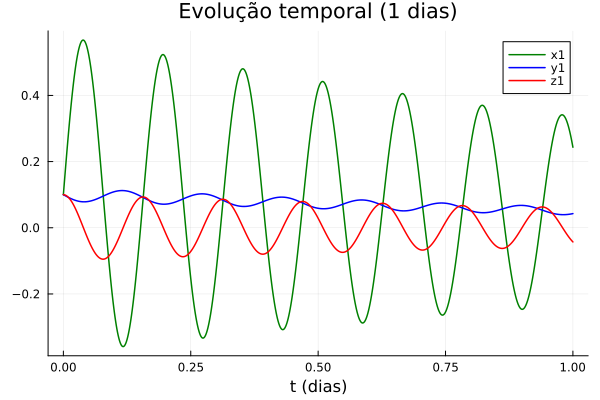
\includegraphics[width=0.85\textwidth]{00_TCC/01_LATEX/figuras/ch01_lorenz_80/evolucao_temporal_01.png}
  \caption{Simulation of the PE model (1 day).\label{fig:lorenz80_pe_1}}
\end{figure}
\begin{figure}[H]
  \centering
    
\includegraphics[width=0.85\textwidth]{00_TCC/01_LATEX/figures/ch01_lorenz_80/temporal_evolution_10.png}
  \caption{Simulation of the PE model (10 days)\label{fig:lorenz80_pe_2}}
\end{figure}
